\newpage
\section{Grundlagen}\label{Grundlagen}
Im folgenden Kapitel werden grundlegende Konzepte und Technologien in den Bereichen Serviceroboter, Webanwendungen, 3D-Modelle und Softwarequalität vorgestellt.

\subsection{Serviceroboter}
Dieser Abschnitt gibt einen kurzen Überblick über Serviceroboter im Allgemeinen und eine Einführung in die Funktionen der Roboter, die in dieser Arbeit eingesetzt werden. Außerdem wird das \ac{BCB} genauer erläutert.

\subsubsection{Definition}
In wissenschaftlichen Arbeiten wird mit vielen verschiedenen Definitionen für Serviceroboter gearbeitet. In dieser Arbeit wird die Definition aus der ISO Norm 8373:2021 \cite[Kap.~3]{ISO2021} verwendet. Nach dieser handelt es sich bei Servicerobotern um Roboter, die im privaten oder professionellen Gebrauch für Menschen nützliche Aufgaben erledigen. Serviceroboter werden hierbei von Industrierobotern und Medizinrobotern abgegrenzt. Die \ac{IFR} \cite{IFR2024} ergänzt die Voraussetzung, dass Serviceroboter voll- oder zumindest teilautonom handeln können. Unter dem professionellen Gebrauch versteht man den kommerziellen Einsatz \cite[S.~4]{GonzalezAguirre2021}, unter anderem im Gesundheitswesen, in der Landwirtschaft oder im Tourismus \cite[S.~9]{GonzalezAguirre2021}.

\subsubsection{Einsatzmöglichkeiten}
Serviceroboter werden bereits vielfältig professionell eingesetzt. So gibt es verschiedene Beispiele in denen sie in Hotels für den Gästeempfang, den Check-in und die Gepäcklieferung und an Flughäfen für die Beratung von Reisenden, das Scannen von Boardingpässen, den Check-in, die Bodenreinigung und Patrouillengänge genutzt werden \cite[S.~425]{Paluch2020}. In der Pflege können Serviceroboter den Pflegern beim Heben von Patienten und beim Durchführen von Übungen mit Patientengruppen aushelfen \cite[S.~427]{Paluch2020}. Aufgaben mit geringer kognitiver und emotionaler Komplexität können in der Regel vollautonom und ohne Aufsicht eines Menschen durchgeführt werden \cite[S.~429]{Paluch2020}. Unter solche Aufgaben fällt zum Beispiel Staubsaugen, Rasenmähen oder Gepäckliefern. Komplexere Aufgaben erfordern die Aufsicht oder Unterstützung von Menschen, wodurch diese nur teilautonom ausgeführt werden \cite[S.~430-431]{Paluch2020}. Für den Einsatz von Servicerobotern müssen immer die Vor- und Nachteile verglichen werden. So können zum Beispiel Roboter, die im Kontakt mit Kunden eingesetzt werden, Emotionen vorspielen, die von Kunden allerdings als unauthentisch erkannt werden. Gleichzeitig sind Roboter im Gegensatz zu Menschen dafür aber ununterbrochen freundlich.\cite[S.~427]{Paluch2020}

\subsubsection{Pudu Robotics}
Diese Arbeit beschäftigt sich mit Robotern von Pudu. Pudu stellt Serviceroboter her, die vor allem in der Gastronomie eingesetzt werden können. Die Modelle sind hierbei auf unterschiedliche Funktionen, wie das Begrüßen von Gästen, das Liefern bestellter Speisen, das Zurückbringen dreckigen Geschirrs und das Putzen des Bodens spezialisiert \cite{PUDU2024}. Damit die Roboter diese Funktionen ausführen können, müssen sie eigenständig durch komplexe, sich ändernde Umgebungen navigieren. Die eigenständige Navigation lässt sich in die Teilfunktionen Positionsfindung, Wahrnehmung und Routenplanung aufteilen, wobei die Positionsfindung eine Schlüsselrolle spielt \cite{Nature2022}. Zur Positionsfindung erstellen sich die Pudu Roboter mit dem sogenannten \ac{VSLAM} eine Karte ihrer Umgebung, was bei einer Fläche von 1000 Quadratmetern eine Stunde dauern kann. Während Roboter zur Navigation normalerweise platzierte Markierungen benötigen, können sich Pudu Roboter mithilfe einer nach oben gerichteten Kamera anhand der Zimmerdecke orientieren.\cite{Pudu2023} Durch weitere Kameras und Sensoren können die Roboter außerdem ihre Umgebung wahrnehmen \cite{Nature2022}.

\subsubsection{Bot Control Backend}\label{sec:BotControlBackend}
Im Rahmen dieser Arbeit wird das bereits existierende \ac{BCB} als Schnittstelle zwischen den Pudu Robotern und dem Prototyp genutzt, über die die Roboter zum Beispiel beauftragt werden können. Die folgenden Informationen zum Service Framework der Roboter stammen aus dem SDK Guidance Document \cite{PuduSDK}, das der Tobit Laboratories AG durch Pudu zur Verfügung gestellt wurde.

Die Abbildung \ref{fig:BotControlBackendCommunication} veranschaulicht die Kommunikation zwischen dem \ac{BCB} und den Robotern. Wie man in der Abbildung sieht hat das \ac{BCB} eine direkte Verbindung zum \gls{Microservice}, der wiederum über die PUDU Cloud – die als \gls{MQTT-Broker} agiert – mit den Robotern kommuniziert. Über \gls{HTTP}-Anfragen an den \gls{Microservice} können Daten abgefragt und Befehle gegeben werden. Bei der Anfrage von Daten fragt der \gls{Microservice} die entsprechenden \gls{MQTT}-Topics an. Wie die Kommunikation zwischen \gls{Microservice} und Robotern funktioniert, wenn das \ac{BCB} Befehle an die Roboter verschickt, ist aus dem Dokument nicht ersichtlich. Die Roboter können zusätzlich auch unaufgefordert Ereignisse an das \ac{BCB} kommunizieren. Hierfür muss das \ac{BCB} eine Adresse für einzelne Ereignistypen im \gls{Microservice} als \gls{Webhook} registrieren. Der \gls{Microservice} abonniert daraufhin die entsprechende \gls{MQTT-Topic}. So schicken die Roboter auftretende Ereignisse – wie eine Positionsaktualisierung – an die PUDU Cloud, die diese an den \gls{Microservice} weiterleitet, da dieser die \gls{MQTT-Topic} abonniert hat. Der \gls{Microservice} schickt das Ereignis daraufhin als \gls{HTTP}-Nachricht an die als \gls{Webhook} registrierte Adresse im \ac{BCB}.

\begin{figure}[H]
    \caption{Kommunikation zwischen Bot Control Backend und Robotern}\label{fig:BotControlBackendCommunication}
    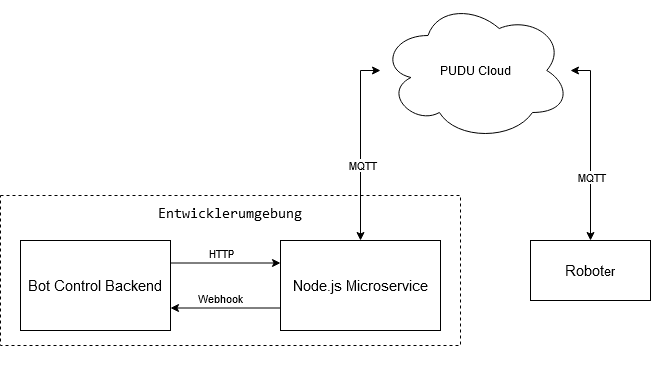
\includegraphics[width=0.9\textwidth]{BotControlBackend Diagramm}
    \\
    Quelle: In Anlehnung an Pudu \cite[S.~4]{PuduSDK}
\end{figure}

Das \ac{BCB} fungiert nicht nur als Kommunikationsschnittstelle zu den Robotern, sondern abstrahiert auch neue Funktionen. So können Roboter mithilfe des \ac{BCB}s Fahrstuhl fahren und somit Lieferpunkte in anderen Stockwerken erreichen. Ebenso können sie durch das \ac{BCB} an geschlossenen Tür halten, diese öffnen und anschließend weiterfahren.

Es gibt verschiedene Daten, die über das \ac{BCB} abgerufen werden können und für den Prototyp relevant sind, wie die Position der Roboter innerhalb ihrer internen Karte, sowie die Positionen wichtiger Standorte wie Lieferpunkte und Ladestationen. Außerdem sind auch die Pfade relevant, an denen sich die Roboter während der Fahrt orientieren. Darüber hinaus sind auch noch die Positionen der virtuellen Wände wichtig. Diese müssen manuell platziert werden und agieren aus der Sicht der Roboter wie echte Wände, wodurch sichergestellt wird, dass bestimmte Bereiche nie durchfahren werden.

\subsection{Webanwendungen}
Webanwendungen sind Softwareanwendungen, die auf Webservern gehostet werden und über Webbrowser aufgerufen werden können. Sie ermöglichen es Benutzern über das Internet auf Anwendungen zuzugreifen, ohne dass eine Installation dieser erforderlich ist. Da sie auf verschiedenen Betriebssystemen und Gerätetypen verwendet werden können, solange ein kompatibler Webbrowser zur Verfügung steht, sind sie plattformunabhängig nutzbar.\cite{AWSWebApp} Zusammenfassend sind Webanwendungen breit und einfach zugänglich.

\subsubsection{Technologien und Softwarebibliotheken}\label{sec:WebTechnologies}
Die reibungslose Entwicklung ansprechender Webanwendungen erfordert den Einsatz verschiedener Technologien.

Die drei zentralen Technologien jeder Webanwendungen sind \ac{HTML}, \ac{CSS} und JavaScript. \ac{HTML} ist eine Auszeichnungssprache, die die Struktur einer Webseite definiert, indem Elemente wie Überschriften, Absätze und Hyperlinks verwendet werden, um Inhalte zu organisieren und zu strukturieren \cite{HTML}. Um das Erscheinungsbild einer Webseite zu gestalten wird \ac{CSS} genutzt. Mit \ac{CSS} lassen sich Layout, Formatierung und weitere Eigenschaften von \ac{HTML}-Elementen definieren.\cite{CSS} \ac{Sass} erweitert \ac{CSS} durch Verschachtelung, Variablen, \gls{Mixins} und weitere Funktionen \cite{Sass}, wodurch die Wiederverwendbarkeit definierter Styles verbessert und die Entwicklung vereinfacht wird. Die Interaktivität von Webseiten wird durch JavaScript ermöglicht \cite{JavaScript}. Bei JavaScript handelt es sich um eine dynamisch typisierte Skriptsprache, die durch TypeScript um eine statische Typisierung erweitert wird \cite{TypeScript}. Durch TypeScript wird die Entwicklung einer robusten und fehlerfreien Webanwendung im Vergleich zu JavaScript erleichtert.

Die Entwicklung komplexerer Webanwendungen wird durch die JavaScript-Bibliotheken React und Redux weiter erleichtert. React wird zur Erstellung von Benutzeroberflächen verwendet und ermöglicht die Entwicklung wiederverwendbarer \ac{UI} Komponenten – im folgenden auch React-Komponenten genannt – sowie eine effiziente Aktualisierung der Benutzeroberflächen durch die Verwendung virtueller \gls{DOM}s. React-Projekte werden in \ac{JSX} entwickelt, womit sich \ac{HTML} Elemente im JavaScript-Code integrieren lassen. Damit React Projekte von Webbrowsern ausgelesen werden können, muss der geschriebene \ac{JSX}-Code zu JavaScript kompiliert werden.\cite{React} Redux ermöglicht eine übersichtliche Verwaltung des Anwendungsstatus \cite{Redux}.

\subsubsection{chayns}\label{sec:Chayns}
Bei chayns handelt es sich um eine Digitalisierungsplattform, die durch die Tobit Software GmbH vertrieben wird. Unter anderem bietet chayns einen Webseiten-Baukasten, mit dem sich Nutzer eine Webpräsenz erstellen können. Auf den Webseiten können vordefinierte chayns Anwendungen, wie ein eShop oder ein Bundesliga-Tippspiel, aber auch eigenentwickelte Webanwendungen eingebunden werden.\cite{chayns} Als Besitzer einer chayns Seite hat man Zugriff auf den Admin-Modus, in dem sich die meisten chayns Anwendungen verwalten lassen. So gibt es auch im entwickelten Prototyp eine Nutzer- und Adminansicht. Tobit bietet verschiedene Softwarebibliotheken, die die Entwicklung von chayns Anwendungen erleichtern. So gibt es den Shell Befehl create-chayns-app \cite{CreateChaynsApp} mit dem chayns basierte React Projekte aufgesetzt werden können; das \ac{npm} Paket chayns-components \cite{ChaynsComponents}, das React-Komponenten für verschiedene \ac{GUI} Elemente zur Verfügung stellt; und das \ac{npm} Paket chayns-api \cite{ChaynsApi}, das verschiedene hilfreiche Funktionen bereitstellt. Für unternehmensinterne Projekte bietet Tobit den \gls{Websocket}-Service der eine indirekte \gls{Websocket}-Verbindung zwischen Backends und Clients ermöglicht. Über diese können Backends unaufgefordert Nachrichten an verbundene Clients versenden.
% chayns.space und chayns toolkit erwähnen

\subsection{3D Modelle}
Dieser Abschnitt bietet eine kurze Einführung in das Thema der 3D-Modelle. Daraufhin werden verschiedene Methoden zur Erzeugung von 3D-Gebäudemodellen vorgestellt und es wird erläutert, wie 3D-Modelle in Webanwendungen eingebunden werden können.

3D-Modelle sind digitale Darstellungen von Objekten oder Szenen in drei Dimensionen. Anders als bei 2D-Grafiken, die lediglich eine Breite und Höhe haben, enthalten 3D-Modelle zusätzlich Tiefeninformationen, aus denen sich die dritte Dimension ergibt. Polygonale 3D-Modelle bestehen aus Polygonen, die sich aus Eckpunkten und Kanten – den Verbindungen zwischen Eckpunkten – zusammensetzen. Oberflächeneigenschaften der Polygone, wie Farben, Glanz und Reflexionen lassen sich durch die Anwendung von Texturen und Materialien definieren. Transformationsoperationen wie Skalierung, Rotation und Translation ermöglichen es, 3D-Modelle im Raum zu bewegen und zu manipulieren. Die Kamera, Perspektive und Projektion legen den Standpunkt des Betrachters und die Darstellung des Modells fest.\cite[S.~8-16]{Parisi2014}

\subsubsection{Generierung}
Neben der manuellen Modellierung von 3D-Modellen, mithilfe von Modellierungssoftware wie Blender, gibt es verschiedene Methoden, die sich insbesondere zur Generierung von Raummodellen eignen.

\paragraph{Fotogrammetrie}

Die Fotogrammetrie beschäftigt sich damit Messungen aus einer Vielzahl an zweidimensionalen Bildern abzuleiten, aus denen sich präzise 3D-Modelle erzeugen lassen \cite[S.~19]{Aber2010}. Inzwischen erfordert die Fotogrammetrie nicht mehr den Einsatz teurer Kameras, da die Kameras moderner Mobilgeräte eine ausreichende Bildqualität bieten \cite{Cohrs2021}. Bei der Planung und Durchführung der Bildaufnahmen müssen verschiedene Aspekte beachtet werden. Innerhalb der aufzunehmenden Szene sollte es eine gleichmäßige Belichtung, möglichst keine reflektierenden oder transparente Flächen und keine sich bewegende Objekte geben. Während der Aufnahme müssen Parameter wie Belichtungszeit und Weißabgleich passend konfiguriert sein und zwischen den einzelnen Aufnahmen unverändert bleiben. Außerdem muss sich der Inhalt aufeinanderfolgender Bilder stets überschneiden.\cite{Cohrs2021b} Nach der Durchführung der Aufnahmen erfolgt die Verarbeitung mithilfe spezialisierter Software, deren Bedienung komplex sein kann. Für eine reibungslose Verarbeitung sind eine leistungsstarke \ac{GPU} und ausreichend Speicherplatz unerlässlich.\cite{Cohrs2021c}

\paragraph{LiDAR Scanning}
Im Gegensatz zur Fotogrammetrie nutzt \ac{LiDAR} einen aktiven Sensor. Es wird Licht in Form eines pulsierenden Lasers ausgesendet. Die Reflexionen werden mit einem Scanner erfasst, wodurch sich Abstände zwischen Sensor und Gegenständen berechnen lassen. Auf Grundlage dieser Messungen wird ein 3D-Modell erstellt. Wie bei der Fotogrammetrie, muss beim Scannen darauf geachtet werden, dass reflektierende oder transparente Flächen, sowie sich bewegende Objekte vermieden werden. Seit 2020 werden \ac{LiDAR}-Scanner in iOS-Geräte von Apple integriert, was zu einer verbesserten Bildqualität beim Fotografieren beitragen soll \cite{Fenstermaker2022}. Als glücklicher Nebeneffekt wurden verschiedene Apps entwickelt, die den \ac{LiDAR}-Scanner nutzen, um 3D-Modelle zu erstellen, wie zum Beispiel Canvas \cite{Canvas2023}, Polycam \cite{Polycam2024} und Scaniverse \cite{Scaniverse2024}. Diese Apps versprechen eine schnelle und einfache Erzeugung akkurater 3D-Modelle.

\paragraph{KI gestützte Methoden}
Es existieren verschiedene \ac{KI}-Modelle, die darauf trainiert sind, 3D-Gebäudemodelle mit nur wenigen Bildern zu erzeugen. Eines dieser \ac{KI}-Modelle ist Plan2Scene. Es benötigt als Eingabe einen Grundriss des Gebäudes, sowie Bilder, die den einzelnen Räumen zugeordnet sind. Basierend auf dem Grundriss generiert das \ac{KI}-Modell ein 3D-Modell mit Möbeln. Basierend auf den Bildern der Räume werden monotone Texturen generiert.\cite[S.~10733]{Plan2Scene2021} Das Rent3D Modell funktioniert ähnlich, nutzt die Bildaufnahmen aber direkt als Textur, statt sie aus den Bildaufnahmen zu generieren \cite[S.~3413]{Rent3D2015}.

\subsubsection{Einbindung im Web}
Das Einbinden von 3D-Modellen wird im Web durch die \ac{WebGL} und WebGPU ermöglicht. Während \ac{WebGL} für lange Zeit der etablierte Standard war, gewinnt WebGPU seit der Veröffentlichung im Jahr 2021 stetig an Popularität.

\paragraph{WebGL und WebGPU}
\ac{WebGL} wurde 2011 von der Khronos Group entwickelt und ist ein JavaScript \ac{API} mit dem 3D-Grafiken im Webbrowser ohne den Einsatz zusätzlicher Plugins dargestellt werden können. Die 3D-Grafiken können hierbei hardwarebeschleunigt angezeigt werden, also über den Einsatz spezialisierter Hardware wie einer \ac{GPU}. Durch die Integration mit \ac{HTML} und JavaScript können 3D-Grafiken dynamisch auf Webseiten eingebunden werden. Da \ac{WebGL} auf offenen Webstandards basiert, ist es in allen Browsern plattformunabhängig nutzbar.\cite[S.~17-19]{Parisi2014} WebGPU bietet wie \ac{WebGL} das hardwarebeschleunigte Anzeigen von 3D-Grafiken und darüber hinaus eine verbesserte Leistung sowie erweiterte Funktionen \cite{Surma2022}. Entwicklern steht eine Vielzahl an Frameworks zur Verfügung die auf \ac{WebGL} oder WebGPU basieren \cite{Seguin2024} und die Entwicklung vereinfachen und beschleunigen.

\paragraph{\deckgl{}}
Das Framework \deckgl{} wurde 2016 von Uber als Open Source Projekt veröffentlicht \cite{Visgl}. Das Framework basiert auf \ac{WebGL}, wobei ab der kommenden Version 9.0.0 stattdessen WebGPU genutzt wird \cite{Green2022}. Mit \deckgl{} lassen sich hochperformante interaktive Karten und Geovisualisierungen mit tausenden bis Millionen Datenpunkten im Web einbinden. Da das Framework auf React ähnlichen Programmierparadigmen basiert eignet es sich besonders gut für die Einbindung in React Anwendungen. Das Framework funktioniert nach dem \ac{PIL} Prinzip. So gibt es Ebenen welche grundlegende visuelle Elemente – im Englischen Primitives –, wie Kreise, Rechtecke und Linien, aber auch komplexere teilweise dreidimensionale Elemente nutzen, um Datenpunkte darzustellen. Die Elemente werden in einer Ebene auf Basis der Attribute der Datenpunkte positioniert, skaliert und gefärbt. Die Ebenen können gestapelt und somit kombiniert werden, was auch die Inspiration für den Namen des Frameworks ist, da das englische Wort deck in etwa Stapel bedeuten kann.\cite[S.~2]{YangWang2019} Das Framework bietet verschiedene vordefinierte Ebenen, wie die IconLayer \cite{DeckglIconLayer}, die Icons als grundlegendes visuelles Element nutzt. Zur Veranschaulichung des \ac{PIL}-Prinzips zeigt die Abbildung \ref{fig:IconLayerExample} wie die IconLayer – in Kombination mit einer weiteren Ebene zur Darstellung der Weltkarte – genutzt wird, um die Positionen aller bekannten Meteoritenlandungen auf der Erde anzuzeigen.

\begin{figure}[H]
    \caption{IconLayer Beispiel}\label{fig:IconLayerExample}
    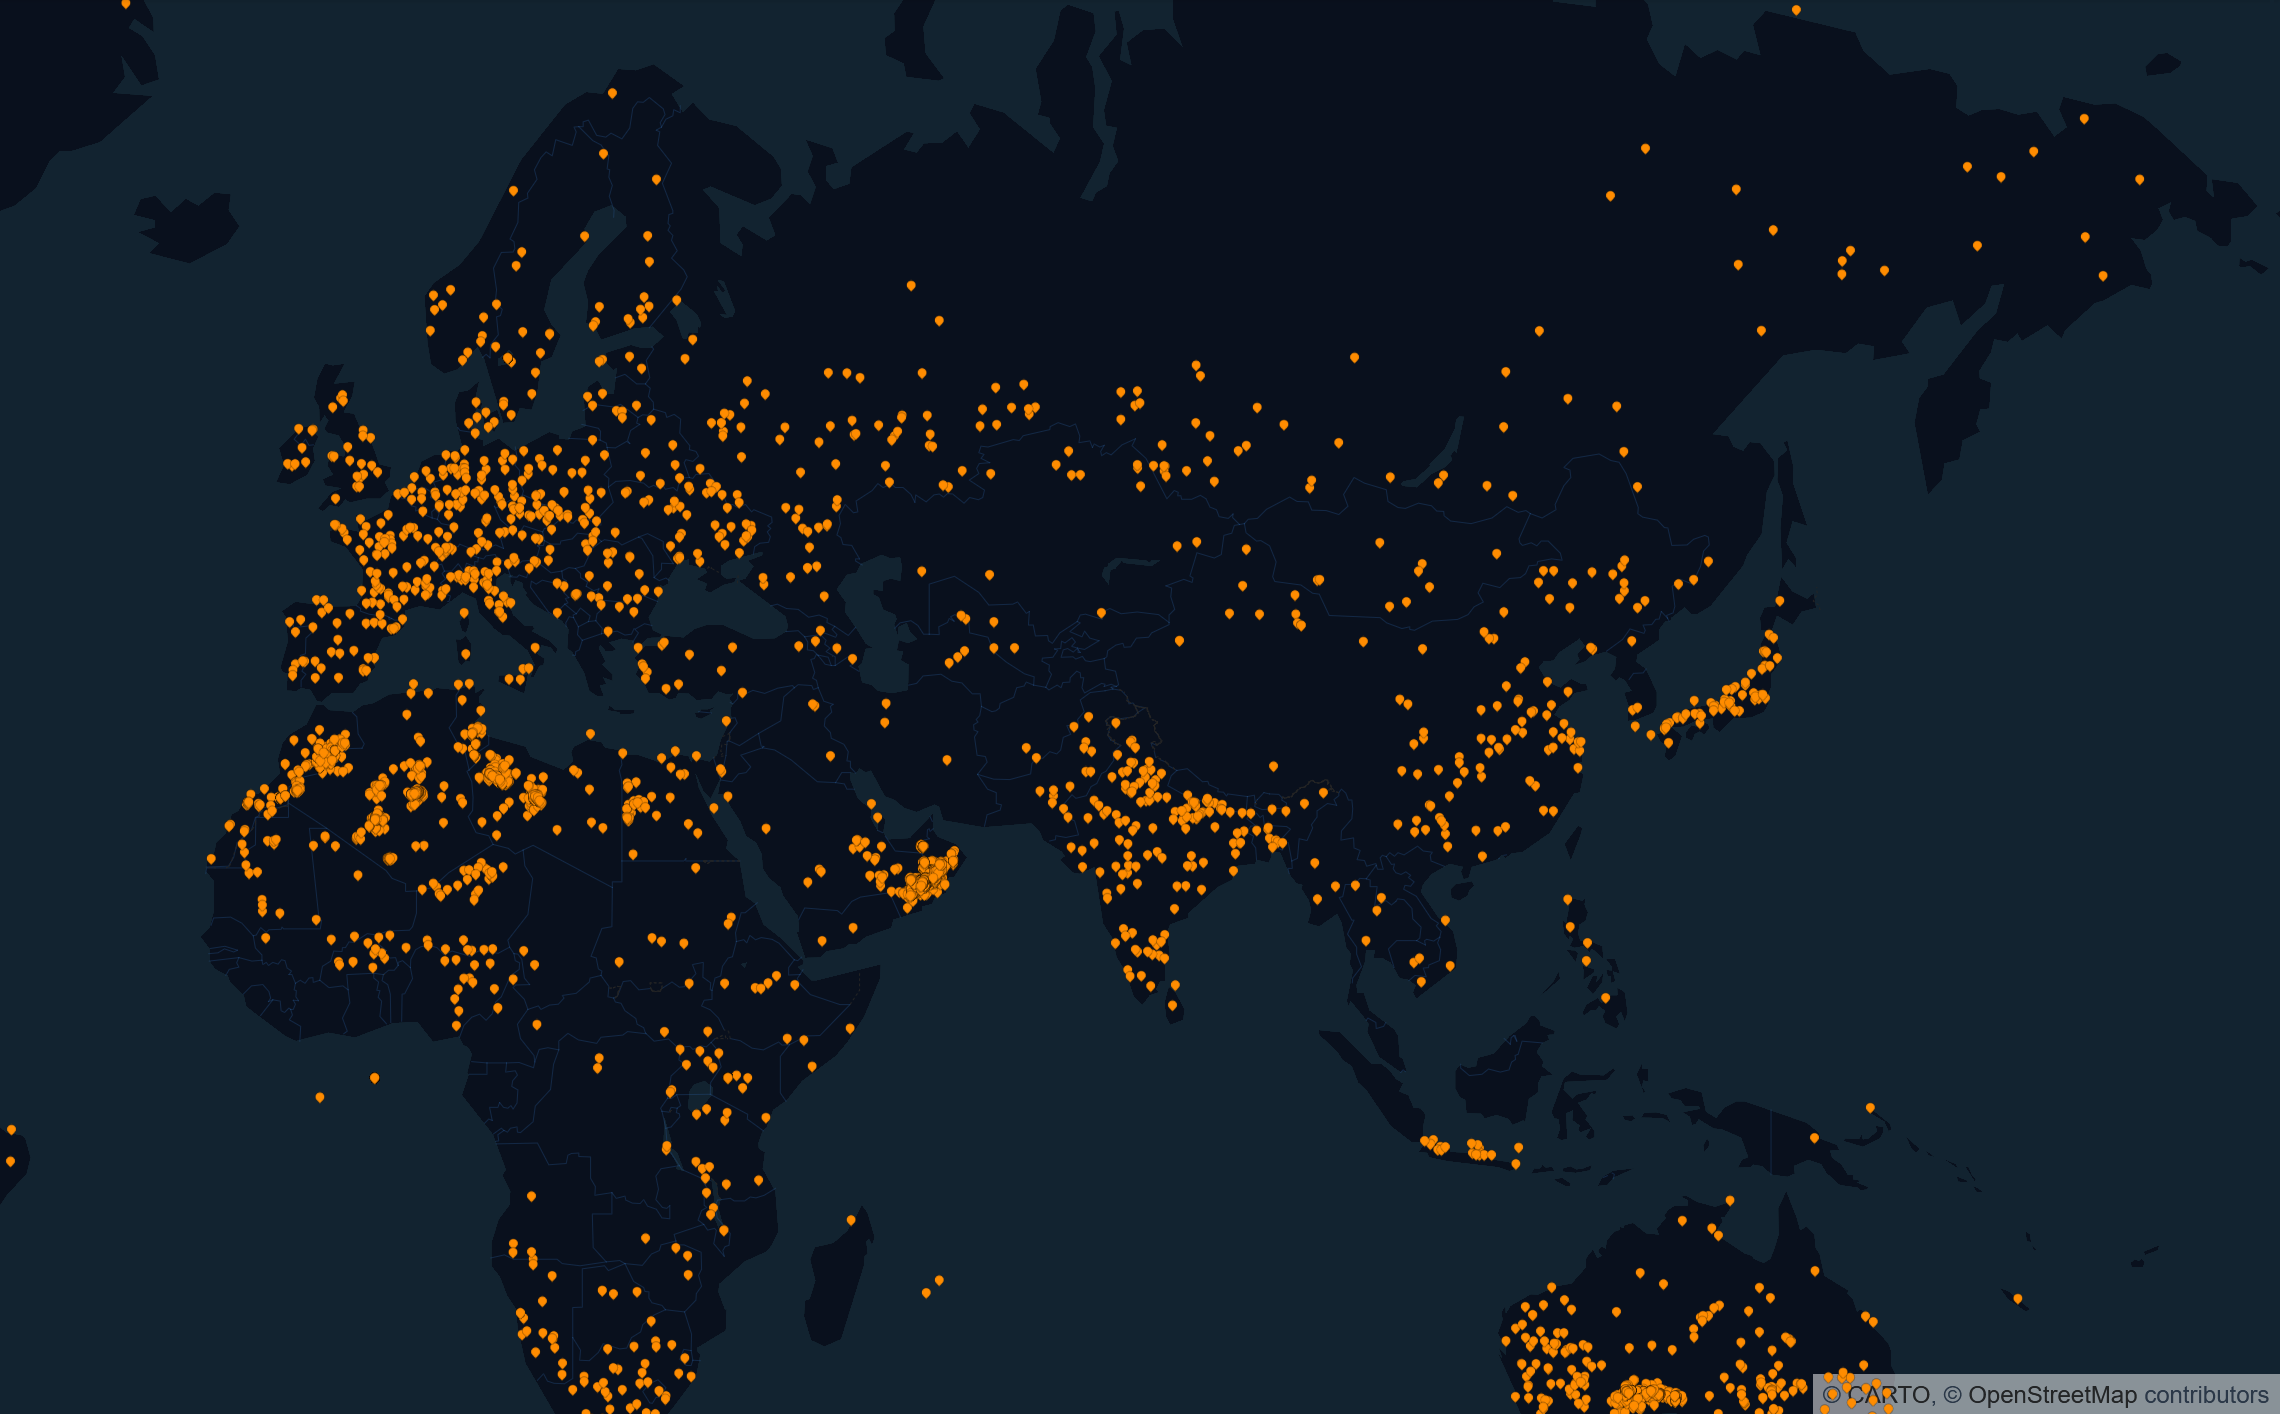
\includegraphics[width=0.9\textwidth]{IconLayer Example.png}
    \\
    Quelle: OpenJS Foundation \cite{DeckGlMeteorites}
\end{figure}

Weitere für diese Arbeit relevante vordefinierte Ebenen sind die SimpleMeshLayer \cite{DeckglSimpleMeshLayer} und ScenegraphLayer \cite{DeckglScenegraphLayer} für das Anzeigen von 3D-Modellen und die PathLayer für das Anzeigen von Pfaden. \deckgl{} bietet auch die Möglichkeit neue Ebenen zu entwickeln, was für diese Arbeit aber nicht relevant ist. Weitere wichtige Elemente die \deckgl{} bietet sind die Controller Klasse \cite{DeckglController}, mit der die Navigation auf der Karte konfiguriert werden kann und die Viewport Klasse \cite{DeckglViewport}, mit der die Navigation direkt kontrolliert werden kann.

\subsection{Softwarequalität}
``Unter Softwarequalität versteht man die Gesamtheit der Merkmale und Merkmalswerte eines Softwareprodukts, die sich auf dessen Eignung beziehen, festgelegte oder vorausgesetzte Erfordernisse zu erfüllen'' \cite[S.~257]{Balzert1998}. So ergibt sich die Softwarequalität aus der Erfüllung der definierten Anforderungen – aber auch aus der Erfüllung der Erwartungen – und zielt darauf ab den Bedürfnissen der Benutzer gerecht zu werden. Diese Anforderungen können in die acht Produktqualitätsmerkmale nach dem ISO-Standard ISO/IEC 25010 eingeteilt werden \cite{ISO25010}. In Abbildung \ref{fig:SoftwareQuality} werden diese Merkmale aufgelistet. Die Merkmale Effizienz und Benutzerfreundlichkeit haben eine besondere Relevanz für diese Arbeit, da sie direkt in der Forschungsfrage gefordert werden. Auch die funktionale Eignung ist relevant, da diese die Erfüllung der funktionalen Anforderungen abdeckt, die im Abschnitt \ref{sec:FunctionalRequirements} definiert werden. Die drei genannten Merkmale sind in der Abbildung entsprechend gekennzeichnet. Im Rahmen dieser Arbeit wird ein Prototyp entwickelt, der nicht die Ansprüche an ein Produktivsystem erfüllen muss. Aus diesem Grund werden die restlichen Merkmale vernachlässigt. Im Folgenden werden die Merkmale Benutzerfreundlichkeit und Effizienz genauer erläutert.

\begin{figure}[H]
    \caption{Qualitätsmerkmale}\label{fig:SoftwareQuality}
    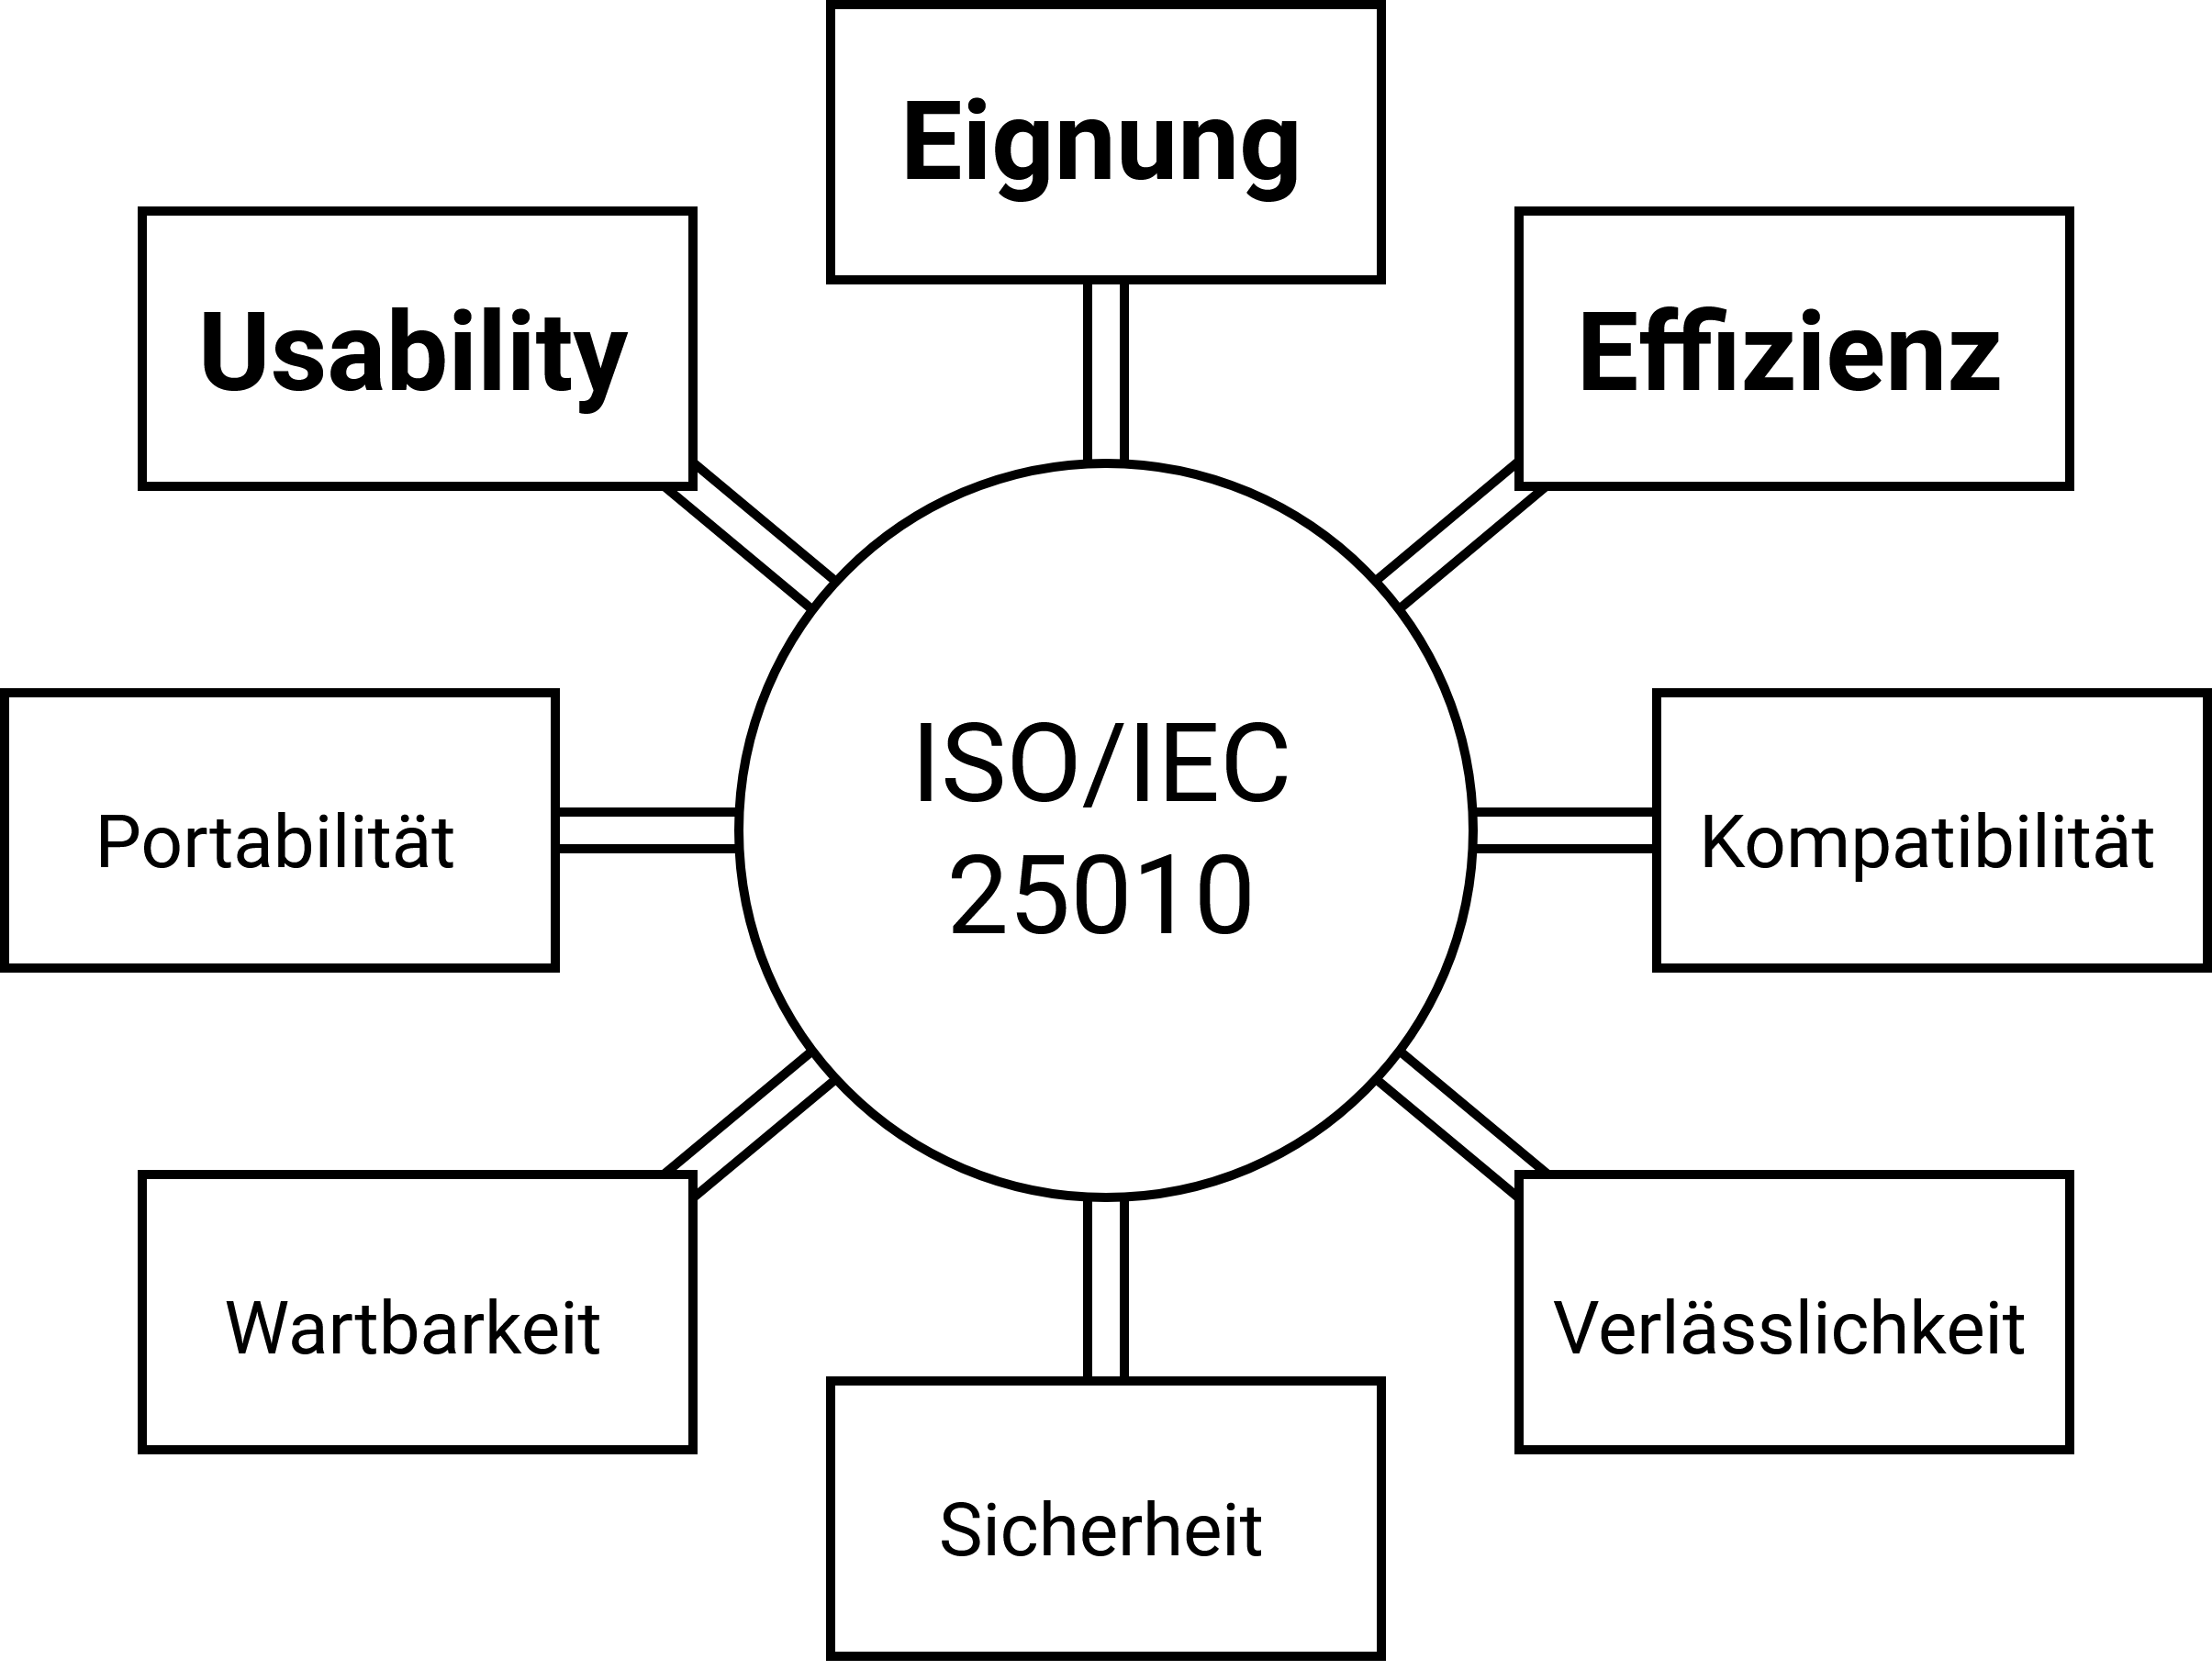
\includegraphics[width=0.9\textwidth]{SoftwareQuality.png}
    \\
    Quelle: Eigene Darstellung
\end{figure}

\subsubsection{Benutzerfreundlichkeit}
Die Benutzerfreundlichkeit wird nach ISO 25010 in sechs Kriterien aufgeteilt: angemessene Erkennbarkeit, Erlernbarkeit, Bedienbarkeit, Toleranz gegenüber Anwenderfehlern, Ästhetik der Benutzeroberfläche und Barrierefreiheit \cite{ISO25010}.

\paragraph{Usability Heuristics}
Die zehn Usability Heuristics von Nielsen sind grundlegende Richtlinien zur Bewertung der Benutzerfreundlichkeit \cite{Nielsen.1994} und decken die ISO 25010 Kriterien weitestgehend ab. So gibt es zum Beispiel die folgenden Richtlinien:

\begin{itemize}
    \item Das Design sollte die Sprache der Benutzer sprechen, indem vertraute Wörter, Phrasen und Konzepte, statt interne Fachbegriffe verwendet werden \cite[Regel 2]{Nielsen.1994}.
    \item Das Design sollte konsistent sein und etablierten Standards folgen, sodass Benutzer nicht darüber nachdenken müssen, ob verschiedene Wörter, Situationen oder Aktionen dasselbe bedeuten \cite[Regel 4]{Nielsen.1994}.
\end{itemize}

Beide Richtlinien helfen dabei das ISO 25010 Kriterium der Erlernbarkeit einzuhalten. Während der Entwicklung können die Richtlinien als Orientierungshilfe dienen, um die Benutzerfreundlichkeit zu verbessern. Eine subjektive Einhaltung dieser ist allerdings unzureichend, um die Benutzerfreundlichkeit zu bewerten. Usability Tests eignen sich hierfür besser.

\paragraph{Usability Tests}
Usability Tests erfordern die Beobachtung von Testpersonen bei der Nutzung des zu prüfenden Produkts, während sie vorab entwickelte Anwendungsszenarien durchspielen. Die Testpersonen sollten potenzielle Benutzer des Produkts repräsentieren.\cite[S.~22]{Dumas.1999} Nach der Durchführung der Tests werden die gesammelten Beobachtungen auf Probleme und Schwachstellen im Produkt ausgewertet. Die Tests können entweder quantitativ oder qualitativ durchgeführt werden. Bei quantitativen Usability Tests werden verschiedene Metriken, wie die Durchführungszeit oder die Rate der erfolgreichen Durchführung von Aufgaben gesammelt. Diese Metriken zeigen im Vergleich zu den Ergebnissen früherer oder zukünftiger Tests, wie sich die Benutzerfreundlichkeit zwischen verschiedenen Versionen entwickelt hat. In qualitativen Usability Tests werden Testpersonen bei der Interaktion mit dem Produkt beobachtet, um Designmerkmale zu identifizieren, die gut oder schlecht zu bedienen sind.\cite{Budiu.2017} Qualitative Tests erfordern einen Moderator, der die Testpersonen durch den Testprozess leitet. Gegebenenfalls gibt es auch weitere Beobachter, die nicht mit den Testpersonen interagieren.\cite{Moran.2019} Für qualitative Tests reicht eine Auswahl an fünf Testpersonen aus, um einen Großteil der Probleme zu finden. Mit einer zunehmenden Menge an Testpersonen sinkt das Return of Investment maßgeblich dadurch, dass immer weniger neue Fehler pro Testperson entdeckt werden.\cite{Nielsen.2012}

\subsubsection{Effizienz}\label{sec:PerformanceBasics}
Die Effizienz einer Anwendung beeinflusst die Benutzerfreundlichkeit und Absprungraten maßgeblich und zeichnet sich unter anderem durch die Dauer der Ladezeiten und die Reaktionsgeschwindigkeit der Benutzeroberfläche aus. Für die Bewertung der Effizienz einer Webanwendung oder Webseite gibt es verschiedene Merkmale. Im Rahmen dieser Arbeit werden der \ac{PLS}, die \ac{LR} und die Smoothness genauer betrachtet. 

Unter dem \ac{PLS} versteht man wie schnell alle visuellen Elemente angezeigt werden \cite{PerformanceMetrics}. Er lässt sich mit dem \ac{LCP} – der Zeit bis das größte oder wichtigste Element angezeigt wird – messen \cite{LCP}. Auch kann mit dem \ac{FCP} gemessen werden, wann das erste Element angezeigt wird \cite{FCP}.

Unter der \ac{LR} versteht man wie schnell der JavaScript Code geladen wird, damit flüssig auf Eingaben des Nutzers reagiert werden kann \cite{PerformanceMetrics}. Gemessen wird diese mithilfe des \ac{FID} Messwerts. Mit diesem wird die Verzögerung gemessen, die bei der ersten Eingabe des Nutzers auftritt \cite{FID}. Außerdem kann die \ac{TBT} gemessen werden, die die Zeit bestimmt, in der der Hauptthread so stark beschäftigt ist, dass die Eingabe-Reaktionsfähigkeit leidet \cite{TBT}.

Mit der Smoothness ist die Geschmeidigkeit gemeint, also ob Übergänge und Animationen mit einer konsistenten Bildrate gerendert werden und flüssig aussehen \cite{PerformanceMetrics}.
